\documentclass[a4paper, 10pt]{article}
\usepackage[utf8]{inputenc}
\usepackage{verbatim}
\usepackage{listings}
\usepackage{graphicx}
\usepackage{a4wide}
\usepackage{color}
\usepackage{amsmath}
\usepackage{amssymb}
\usepackage[dvips]{epsfig}
\usepackage[toc,page]{appendix}
\usepackage[T1]{fontenc}
\usepackage{cite} % [2,3,4] --> [2--4]
\usepackage{shadow}
\usepackage{hyperref}
\usepackage{titling}
\usepackage{marvosym }
\usepackage{subcaption}
\usepackage[noabbrev]{cleveref}

\renewcommand{\topfraction}{.85}
\renewcommand{\bottomfraction}{.7}
\renewcommand{\textfraction}{.15}
\renewcommand{\floatpagefraction}{.66}
\renewcommand{\dbltopfraction}{.66}
\renewcommand{\dblfloatpagefraction}{.66}
\setcounter{topnumber}{9}
\setcounter{bottomnumber}{9}
\setcounter{totalnumber}{20}
\setcounter{dbltopnumber}{9}


\setlength{\droptitle}{-10em}   % This is your set screw

\setcounter{tocdepth}{2}

\lstset{language=c++}
\lstset{alsolanguage=[90]Fortran}
\lstset{basicstyle=\small}
\lstset{backgroundcolor=\color{white}}
\lstset{frame=single}
\lstset{stringstyle=\ttfamily}
\lstset{keywordstyle=\color{red}\bfseries}
\lstset{commentstyle=\itshape\color{blue}}
\lstset{showspaces=false}
\lstset{showstringspaces=false}
\lstset{showtabs=false}
\lstset{breaklines}
\title{FYS3150 - Project 3}
\author{Daniel Heinesen, Gunnar Lange}
\begin{document}
\maketitle
\begin{abstract}We present an investigation into numerical algorithms for solving complex systems of ODE's, by simulating a many-body problem - our solar system, with varying levels of complexity. We present the forward Euler algorithm and the Velocity-Verlet algorithm, and show that, when computation time is not a vital concern, the Velocity-Verlet algorithm outperforms the Forward Euler. We also investigate the appropriate time step to model our system over long time scales, and find that $10^5$ steps per year gives us sufficient numerical precision. Finally, we show that our program largely reproduces some known analytic results, namely conservation of energy/angular momentum, the escape velocity of earth from the sun and the perihelion precession of mercury predicted by general relativity. All data, scripts and plots can be found on our \href{https://github.com/dulte/Comp-Phys/tree/master/Project3Final}{Git-page}\footnote{https://github.com/dulte/Comp-Phys/tree/master/Project3Final}
\end{abstract}
\newpage
\tableofcontents
\newpage
\section{Introduction}
The n-body problem is a recurring theme in many physics publications (see for example \cite{PhysRevLett.19.1312} or \cite{Diacu2012} ), due to complexity and its applicability in fields such as statistical dynamics or astrophysics.  Analytic solutions of these problems are notoriously hard to come by and are, in most situations, unattainable. Therefore, these problems are almost always solved by use of numerical techniques.\\
\linebreak
We present two different numerical methods for solving the coupled ODE's resulting from Newton's gravitational laws - Euler's method and the velocity-Verlet method. We begin by a theoretical introduction to both algorithms, as well as to the equations which we wish to solve. We then discuss some checks which our simulations should pass. Specifically, we look at conservation of energy and angular momentum. We continue by looking at some results which have analytic solutions from physics - specifically the escape velocity of earth from the solar system and the perihelion precession of mercury predicted by general relativity. We compare our model to these results, as another check for consistency. We also investigate what parameters to use in our algorithms to get consistent numerical results.\\
\linebreak
We then briefly present the methods we used to implement these algorithms, as well as presenting the various models we investigated. Subsequently, we present our results and discuss these.
\section{Theoretical model}\label{Theoretical_section}
In this section, we introduce the quantities and equations required to model the solar system. We begin by introducing the relevant equations, and subsequently discuss how to solve these numerically. We continue with a brief discussion of the units used, followed by a discussion of tests that we can implement to test our numerical results. We conclude with a brief diversion to relativistic effects in the solar system.
\subsection{Newtonian Gravity}\label{Newtonian_Gravity}
Newton's general law of gravitation, which describes the force of gravity between two objects, is given by:
\begin{equation}
\vec{F}_{G}=\frac{Gm_1m_2}{r^3}\vec{r}
\end{equation}
Here $F_G$ is the force of gravity on the first mass, $G$ is the universal gravitational constant, $m_i$ are the masses of the two objects, and $\vec{r}$ is the vector pointing from $m_1$ to $m_2$. This law can be combined with Newton's second law of motion, to give a set of coupled differential equations:
\begin{equation}\label{eq:coupled_diff}
\begin{split}
\frac{d^2x}{dt^2}=\frac{F_{G,x}}{m_1}\\
\frac{d^2 y}{dt^2}=\frac{F_{G,y}}{m_1}\\
\frac{d^2 z}{dt^2}=\frac{F_{G,z}}{m_1}\\
\end{split}
\end{equation}
Where $F_{G,x}, F_{G,y}$ and $F_{G,z}$ are the components of the gravitational force in the $x, y$ and $z$ directions respectively. These equations can be reduced to a set of first-order equations by introducing the velocity components, $v$, such that:
\begin{equation}\label{eq:Velocity_position_equation}
\frac{dx}{dt}=v_x, \quad \quad \frac{dv_x}{dt}=\frac{F_{G,x}}{m_1}=a_x(x,y,z)
\end{equation}
And equivalently for the $y$ and $z$ direction. This gives six coupled, first-order, linear, differential equations.
\subsection{Implementing the initial conditions}\label{implement_IC}
To find a unique solution of the set of equations in section \ref{Newtonian_Gravity}, we require some initial conditions, i.e. some $x(t=0)$, $v_x(t=0)$, and equivalently for the $y$ and $z$ direction. For our first model (described in section \ref{First_model}) we will, for simplicity, let the earth be $1$ AU away from the sun, with an initial velocity that ensures a circular orbit. We show in appendix \ref{ap:Find_Circular_orbit} that this results in the requirement that the initial velocity be given by:
\begin{equation}
v_0=\sqrt{\frac{GM_{\odot}}{r}}
\end{equation}
Where $M_{\odot}$ is the mass of the sun and $r$ is the distance to the sun.\\
\linebreak
For the subsequent models, with multiple planets, we will use the initial positions and velocity provided on NASA's \href{http://ssd.jpl.nasa.gov/horizons.cgi#top}{webpages}\footnote{http://ssd.jpl.nasa.gov/horizons.cgi\#top}, letting $t=0$ correspond to the 18th of October 1977 (right before the launch of Voyager 2, as an arbitrary start point).\\
\linebreak
We want to ensure that the center of mass of our solar system is stable at the origin. On NASA's webpage, we can choose the coordinate origin, however, it is not entirely clear if the velocities have been adjusted so that the center of mass is at rest. Therefore we adjusted the position and velocity of the sun to accommodate this. The position vector of the center of mass, $\vec{R}_{COM}$, is found from:
$$\vec{R}_{COM}=\sum_i m_i\vec{r}_i$$
The sum is over all bodies. $\vec{r}_i$ is the position vector of body $i$,  and $m_i$ is its mass. As the sun is by far the heaviest mass in the system, we can ensure that $\vec{R}=\vec{0}$ by letting the position vector of the sun, $\vec{r}_{\odot}$ be given by:
$$\vec{r}_{\odot}=-\frac{\sum_j m_j\vec{r}_j}{M_{\odot}}$$
Where the sum is over all bodies \textit{except the sun}. We can do the same thing for the velocity of the center of mass, $\vec{V}_{COM}$, which is given by:
$$\vec{V}_{COM}=\sum_i m_i \vec{v}_i$$
Where $\vec{v}_i$ is the velocity of body $i$. We can then let the velocity of the sun, $\vec{v}_{\odot}$ be:
$$\vec{v}_{\odot}=-\frac{\sum_j m_j\vec{v}_j}{M_{\odot}}$$
Where the sum is again over all bodies \textit{except} the sun. This ensure that the center of mass of our system is fixed at the origin.
\subsection{Discretizing the equations}\label{discretize_equations}
We will solve the equations in \ref{eq:coupled_diff} numerically. Therefore we require discretized versions of the these equations. We want to simulate from $t=t_0$ to $t=t_f$, and choose $N$ evenly spaced points in this interval. This gives us a timestep, $h$, of:
$$h=\frac{t_f-t_0}{N}$$
Let now $t_i=a+ih$, where $i$ goes from $0$ to $N$. Furthermore, let $x_i=x(t_i)$ and $ v_{x,i}=v_x(t_i)$, and equivalently for the $y$ and $z$ direction. Finally, discretize the acceleration as $a_{x,i}=a_x(x_i, y_i, z_i)$. This allows us to discretize the derivatives in equation \ref{eq:Velocity_position_equation}. We will do this in two separate ways; with the forward Euler algorithm and with the Velocity-Verlet algorithm.
\subsubsection{Euler's forward method}
Euler's forward algorithm amounts to discretizing the derivatives from section \ref{Newtonian_Gravity} as:
\begin{equation}\label{eq:Euler_Forward}
\frac{dg}{dt}\approx \frac{g_{i+1}-g_i}{h}
\end{equation}
This approximation is based on Taylor-expanding the function $g(t)$ to the second order, as explained by \cite{Forward_Euler}. Inserting this approximation for the derivatives in equation \ref{eq:Euler_Forward}, and rearranging some of the terms, gives:
\begin{equation}
\begin{split}
v_{x, i+1}=v_{x,i}+ha_{x,i}\\
x_{i+1}=x_i+hv_{x,i}
\end{split}
\end{equation}
And again equivalently for the $x$ and $y$ direction. This is the Euler forward algorithm. Combining this with the initial conditions, $\vec{v}(t_0)=\vec{v}_0$ and $\vec{x}(t_0)=\vec{x}_0$, makes it possible to solve the equations of Newtonian gravity. Closer inspection (through Taylor expansion, see for example \cite{Error_Euler}), reveals that the local error is proportional to $h^2$, whereas the global error is proportional to $h$. Thus, whilst this is a straightforward algorithm, the errors quickly accumulate. It is therefore of interest to investigate a slightly improved algorithm:

\subsubsection{Velocity-Verlet Algorithm}
The Velocity-Verlet algorithm is based on the idea of Taylor-expanding the acceleration, in addition to the velocity and position. The details can be found in appendix \ref{ap:Deriving_VelVer}, but the method produces the following equations:
\begin{equation} \label{eq:Vel_Ver_eq}
\begin{split}
x_{i+1}=x_i+hv_{x,i}+\frac{h^2}{2}a_{x,i}\\
v_{x,i+1}=v_{x,i}+\frac{h}{2}\left(a_{x,i+1}+a_{x,i}\right)
\end{split}
\end{equation}
And similarly for the $x$ and the $y$ equations. Note that $a_{i+1}$ depends on $x_i, y_i$ and $z_i$, and therefore all three position coordinates must be computed before we can compute the velocity. As shown in our analysis in appendix \ref{ap:Deriving_VelVer}, the local error is proportional to $h^3$, and in turn the global error is proportional to $h^2$, as discussed by \cite{Global_VV}. \\
\linebreak
Notice that $a_{x i+1}$ can be reused in the next step, so this method does not incur any additional calls to the acceleration function in the main loop, as compared to the Forward Euler algorithm. The method only costs a few more FLOPs;
\begin{itemize}
\item We must perform two additional multiplications for each dimension, specifically $(h^2/2)\cdot a_{x,i}$ and $(h/2)\cdot a_{x, i+1}$
\item We must perform two further additions per dimension, namely adding $(h^2/2)a_{x,i}$ and $(h/2)a_{x, i+1}$ to respectively $x_{i+1}$ and $v_{x, i+1}$.
\end{itemize} 
This gives four additional FLOPs per timestep and dimension, i.e. 12 FLOPs per timestep. Thus if we have $N$ points in the main-loop, this gives an additional $12N$ FLOPs. Note that $h^2/2$ and $h/2$ can be precomputed, and therefore do not contribute to the number of FLOPs in the main loop. 
\subsection{Choice of units}
As we will be modelling our solar system, a natural unit of length is the average distance between the earth and the sun, the astronomical unit, AU. In SI-units, $1 \mathrm{AU} \approx 1.496 \cdot 10^{11} \mathrm{m}$. As the most massive object in the solar system is the sun, we choose one solar mass, $M_{\odot}$ as our mass unit. In SI units, $M_{\odot} \approx 1.99 \cdot 10^{30}$. We will use the mean tropical year, which is about 365.24 days of 864000 seconds (\cite{Tropical_year}). This choice of units has one considerable advantage - it simplifies the expression for the gravitational constant, $G$. As shown in appendix \ref{ap:Find_Circular_orbit}, with this choice of units the gravitational constant becomes:
$$G=4\pi^2 \ \mathrm{AU^{3}yr^{-2}M_{\odot}^{-1}}$$
As discussed in section \ref{GR_section}, we will also use the speed of light. With our units, this is given by:
$$c=63\ 198 \ \mathrm{AU/yr}$$
\subsection{Conserved quantities in the system}\label{conservation_of_energy}
To check the consistency of our results, we will investigate whether certain quantities, which we expect to be conserved, are indeed conserved.
\subsubsection{Conservation of mechanical energy}
As there are no external forces in the system, we expect the mechanical energy to be conserved. There are two kinds of energy to consider in our system: kinetic and potential energy. The kinetic energy of a single body is simply given by:
$$E_{k}=\frac{1}{2}mv^2$$
Where $m$ is the mass of our celestial body and $v$ is the absolute value of its velocity. This is the standard formula for the kinetic energy. The potential energy can be found by integrating the force, choosing infinity as a reference point, i.e. $U(\infty)=0$:
$$U=-\int_r^{\infty} \frac{GMm}{r'^2} dr'=-\frac{GMm}{r}$$
This is the potential energy between the bodies. Thus the total energy (which should be conserved) is given by:
\begin{equation}\label{eq:total_energy}
E_{tot}=\sum_{i} \frac{1}{2}m_iv_i^2 - \sum_{i<j}\sum_{j}\frac{Gm_im_j}{r_{ij}}
\end{equation}
Where $i$ runs over all the bodies and $r_{ij}$ is the norm of the distance between body $i$ and $j$. Note that the second sum of the potential energy only goes to $i<j$, to avoid double-counting the energy.
\subsubsection{Conservation of angular momentum per unit mass}
As there is no external force, there is also no external torque. Therefore, the net angular momentum per unit mass should be conserved in our system. The angular momentum per unit mass of a body is generally given by:
$$\vec{l}=\vec{r}\times \vec{v}$$
Where $\vec{v}$ is the velocity of the body, and $\vec{r}$ is the distance to the center of mass. The total angular momentum per mass is then is then:
\begin{equation}\label{eq:total_angular_momentum}
\vec{l}_{tot}=\sum_i \vec{r}_i\times \vec{v}_i
\end{equation}
Where the sum is over all bodies.\\
\linebreak
Equations \ref{eq:total_energy} and \ref{eq:total_angular_momentum} both describe quantities which should be conserved. Thus, an important consistency check for our code, is to test if these quantities are indeed (approximately) constant throughout our simulation.
\subsection{Escape velocity}\label{escape_vel_section}
Another way we can check the consistency of our results is to investigate the escape velocities of the planets. This can be done by equating the potential energy to the kinetic energy. This is a difficult problem for a many-body problem. Therefore, we will only implement this in  the two-body case, with the sun and the earth. Equating potential and kinetic energy of the earth gives: 
$$\frac{1}{2}v_{esc}^2=\frac{GM_{\odot}}{r}$$
Solving:
\begin{equation}
v_{esc}=\sqrt{\frac{2GM_{\odot}}{r}}
\end{equation}
Which is the escape velocity of the earth, if we ignore the other planets. In our units, $v_{esc} = 2\sqrt{2}\pi\ \mathrm{AU/yr} \approx 8.89 \ \mathrm{AU/yr}$. We can experiment with the initial velocity of our planets, and check if the velocity at which a planet manages to escape equals this quantity. This gives us another way to check the consistency of our results.
\subsection{The perihelion precession of Mercury}\label{GR_section}
One of the tests for Einstein's theory of relativity is the perihelion precession of Mercury.  Over time, the perihelion (the point where Mercury is closest to the sun) changes. This was initially thought to be due to the gravitational attraction of other planets, but the effect was too large.It turns out that this effect is due to general relativity, which predicts that gravity warps spacetime. This boils down to modifying the gravitational force to:
\begin{equation}\label{eq:GR_equation}
\vec{F}_G=\frac{GM_{\odot}M_{\mathrm{Mercury}}}{r^3}\left[1+\frac{3l^2}{r^2c^2}\right]\vec{r}
\end{equation}
Where $l=|\vec{l}|$ is the absolute value of the angular momentum per mass of the body the force acts on, and $c$ is the speed of light. This assumes that all other effects, such as gravitational attraction from other planets, have been ignored. In this case, experimental data shows that the perihelion angle precesses $43''=0.2085\  \mathrm{mrad}$ per 100 earth years. We will investigate if this relativistic correction can correctly predict the precession, by comparing the motion of Mercury (removing all other planets) with Newtonian gravity and with the relativistic expression for gravity.
\newpage
\section{Methods}
In this section we give an overview of the methods that we employed to solve the problems outlined in the previous sections. We discuss the models we have implemented, the numerical implementation of these models and the equations from the previous section and finally the implementation of initial conditions.
\subsection{Models}\label{models}
We will implement four different models, to test our simulations under multiple circumstances. 
\subsubsection{First model - The earth-sun system}\label{First_model}
We begin with a simplified model of our solar system, containing only the earth and the sun. We simulate this using both the Euler forward algorithm and the Velocity-Verlet algorithm, which enables us to compare these methods. 
\subsubsection{Second model - The three body problem}
We slightly expand our system by also including the most massive planet - Jupiter. We can then investigate how large the effect of Jupiter is on the orbit of the earth. We will also make this slightly more extreme, by increasing the mass of Jupiter by a factor $10$ and a factor $1000$. In the latter case, we will be approaching a binary star system, as the mass of Jupiter is about $1000$ times less than the mass of the sun. Thus we expect a fairly chaotic behavior, which will allow us to study the stability of our Verlet solver.
\subsubsection{Third model - Entire solar system}
We then include all eight planets in the solar system, as well as Pluto for historical reasons. We also include all interactions between the planets. We use the Velocity-Verlet method to solve this numerically, which gives us an opportunity to study the stability of the Verlet-method on larger scales.
\subsubsection{Final model - The mercury-sun system}
Finally, we model only mercury and the sun, to investigate the perihelion precessions of mercury described in section \ref{GR_section}. Here we use the Verlet-solver, and implement both the Newtonian and the relativistic expressions for the gravitational force.
\subsection{Some interesting features of our numeric scripts}
\subsubsection{Data flow}
To ease the flow of data, we implement a class structure to our code. We have three interacting classes:
\begin{enumerate}
\item Particle class - a class which stores all variables related to a single planet.
\item System class - A class which stores all and computes all species related to the entire system.
\item ODESolver class - A class which computes acceleration based on the algorithms detailed in section \ref{discretize_equations}
\end{enumerate}
Finally we also implement a tailored vector class, which implements some key features of vector algebra needed to solve the equations in section \ref{Newtonian_Gravity}, such as addition, multiplication, norms, inner products and the cross product.
\subsubsection{Retrieving the initial conditions}
As described in section \ref{implement_IC}, the initial positions and velocities of all planets can be retrieved from NASA's  \href{http://ssd.jpl.nasa.gov/horizons.cgi#top}{webpages}. It is possible to establish a telnet connection to these websites, and retrieve the data automatically. We took inspiration from \cite{NASA} when implementing this.\\
\linebreak
\linebreak
With the class structure and the initial conditions in place, we can then simply initialize the solar system by a code akin to the one shown below:
\lstinputlisting{Pseudo_code_make_planets.py}
And then we can simply solve the differential equations by calling:
\lstinputlisting{Pseudo_code_solve_system.py}

\subsection{Checking the consistency of our results}
\subsubsection{Checking conservation of energy and angular momentum per unit mass}
We check conservation of energy for every 10$0^{th}$ timestep in all of the models described in section \ref{models}, except for the case with relativistic gravity. As our background in general relativity is relatively limited, we are unsure whether or not energy and angular momentum per mass are conserved in this case.\\
\linebreak
Because magnitudes of deviations are notoriously difficult to interpret, we will instead record and analyze the relative error at a time, $t$, defined as:
\begin{equation}\label{eq:relative_error}
\epsilon_{rel}=\frac{E(t)-E_{\mathrm{initial}}}{E_{\mathrm{initial}}}
\end{equation}
Where $E$ is the energy. We employ the same expression to check conservation of angular momentum per unit mass.
\subsubsection{Checking escape velocity}
We found an expression for the escape velocity in section \ref{escape_vel_section}. To show that this indeed gives the required behavior, we place the earth at $x=1\ \mathrm{AU}$ and give it an initial velocity in the y-direction. We let this initial velocity be just above and just below the escape velocity, and investigate the behavior of the system.
\subsubsection{Checking the precision of the Velocity-Verlet method}
As we mentioned in section \ref{discretize_equations}, the Velocity-Verlet method is significantly more precise than the forward Euler algorithm. We therefore investigate the stability of the Velocity-Verlet method for a variety of timesteps, and simulate for two years, to investigate when the two graphs of the two years are acceptably close. This will enable us to choose a sensible time step for our simulations.
\subsection{Investigating the perihelion processions of mercury}
To find the perihelion processions of mercury, we must develop an algorithm which checks for a minimum of the distance between the sun and mercury. We do this by storing the absolute value of the position vector for three different timesteps, and subsequently check if the value in the middle of these three is lower than the two others. If this is the case, we save it as a perihelion passing, and compute the angle. This is illustrated in the pseudo-code below:
\lstinputlisting{Pseudo_code_perihelion.py}
\newpage

\section{Results}
In this section we present the orbits of the different models, as well as quantities such as conservation of energy/momentum and escape velocity/perihelion precession. Our calculations were all done in 3D, but we include only 2D plots, as these are easier to interpret. The orbits of all planets, except Pluto, are almost two-dimensional anyway, as can be seen from the solar\_system\_3D.gif file on our \href{https://github.com/dulte/Comp-Phys/tree/master/Project3Final}{GIT-page}\footnote{https://github.com/dulte/Comp-Phys/tree/master/Project3Final}. We postpone an extended discussion of our results until section 5.
\subsection{Results from the first model - Earth-Sun}
\subsubsection{Position}
The position of the earth and the sun, as well as a zoomed-in version of the plot, are shown in the figures below:
\begin{figure}[!ht]
    \centering
    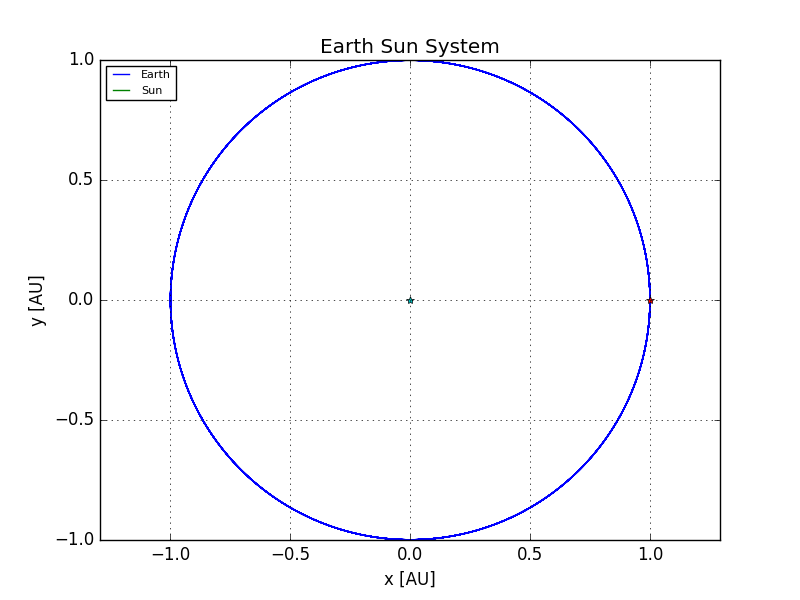
\includegraphics[height=2.5in]{earthsun.png}
    \caption{The earth-sun system, simulated for 10 years, with $10^7$ timesteps per year. We are using the Velocity-Verlet method, though there is no visible difference between the Velocity-Verlet and the Euler method at this scale.} \label{fig:earth-sun-figure1}
\end{figure}


\begin{figure}[!ht]
    \centering
    \begin{subfigure}[H!]{0.5\textwidth}
        \centering
        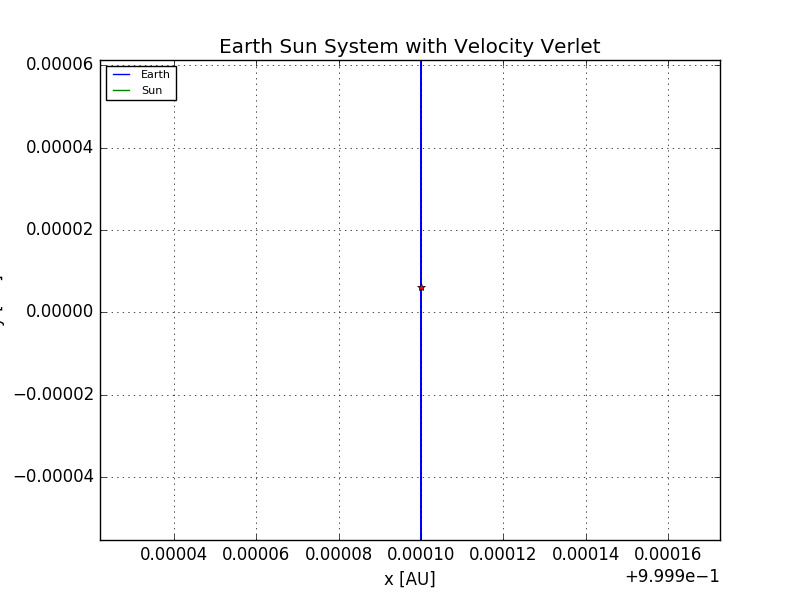
\includegraphics[height=2.0in]{orbitESVV.png}
        \caption{Velocity-Verlet algorithm}
    \end{subfigure}%
    ~ 
    \begin{subfigure}[H!]{0.5\textwidth}
        \centering
        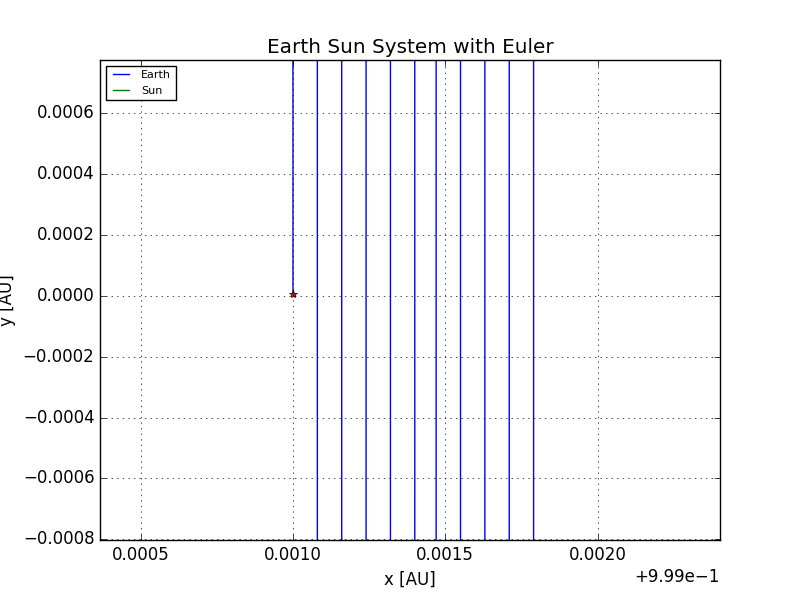
\includegraphics[height=2.0in]{orbitESEuler.png}
        \caption{Euler's forward algorithm}
    \end{subfigure}
    \caption{Zoomed-in version of the figure above with two different solution methods. Note that the scale on subplot $a$ is ten time smaller than the scale of subplot $b$.}
\end{figure}
\subsubsection{Conservation of energy and angular momentum per unit mass}
A plot of the relative error in the total energy and the total angular momentum per unit mass for the Velocity-Verlet and the Euler algorithm is shown below:
\begin{figure}[!ht]
    \centering
    \begin{subfigure}[H!]{0.5\textwidth}
        \centering
        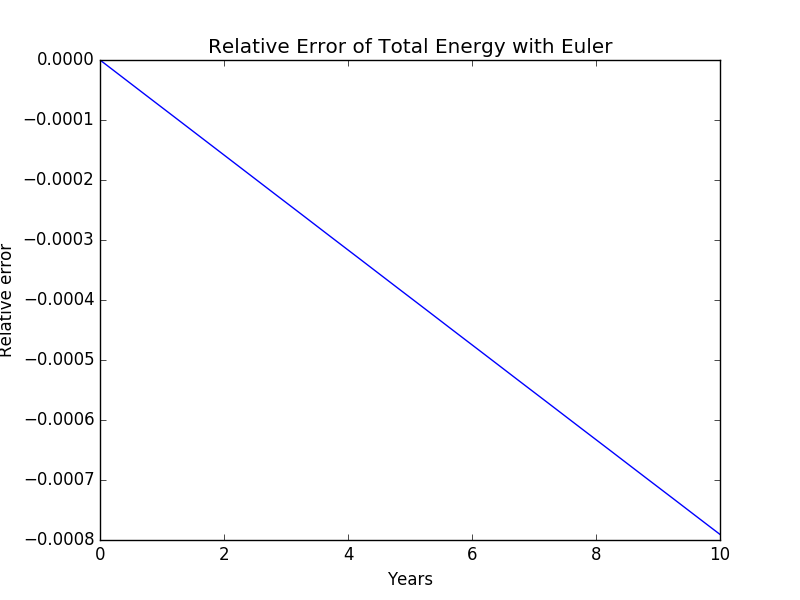
\includegraphics[height=2.0in]{relErrEnESEuler.png}
        \caption{Forwad Euler algorithm}
    \end{subfigure}%
    ~ 
    \begin{subfigure}[H!]{0.5\textwidth}
        \centering
        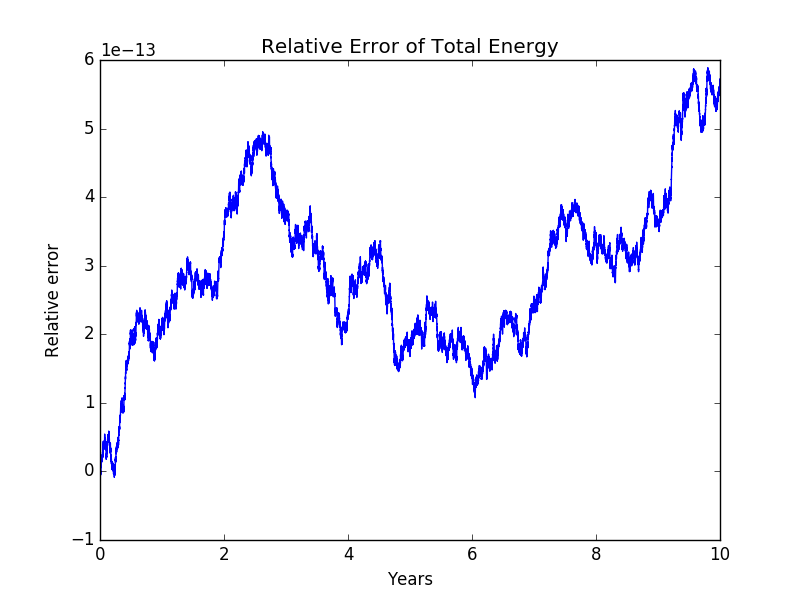
\includegraphics[height=2.0in]{relErEnES.png}
        \caption{Velocity-Verlet algorithm}
    \end{subfigure}
    \caption{Variations in the error of the total energy as a function of time for 10 years of orbit of the earth-sun system. Note the scale on the axis.}
\end{figure}
\begin{figure}[!ht]
    \centering
    \begin{subfigure}[H!]{0.5\textwidth}
        \centering
        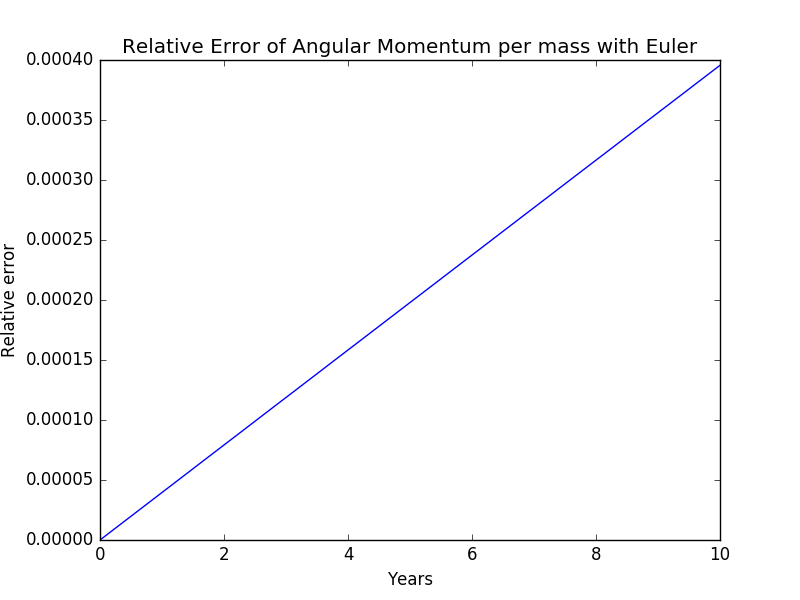
\includegraphics[height=2.0in]{relErrMomESEuler.png}
        \caption{Forwad Euler algorithm}
    \end{subfigure}%
    ~ 
    \begin{subfigure}[H!]{0.5\textwidth}
        \centering
        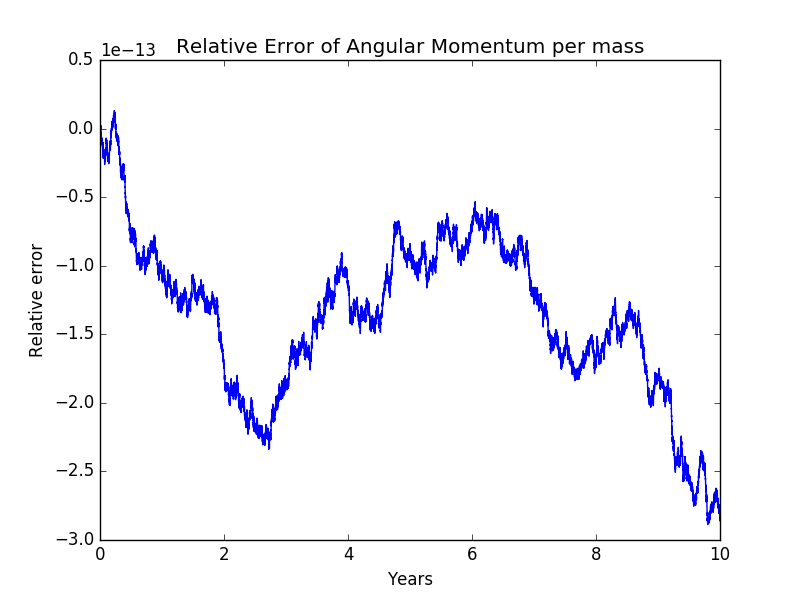
\includegraphics[height=2.0in]{relErMomES.png}
        \caption{Velocity-Verlet algorithm}
    \end{subfigure}
    \caption{Variations in the error of the total angular momentum per unit mass as a function of time for 10 years of orbit of the earth-sun system. }
\end{figure}
\newpage
\subsection{Investigating the time step}
Plots for a variety of a timesteps are shown below. $\Delta t$ is the timestep. Note that a similar plot was already shown for $\Delta t = 10^{-5}$ in figure 2 above. 
\begin{figure}[!ht]
    \centering
    \begin{subfigure}[H!]{0.5\textwidth}
        \centering
        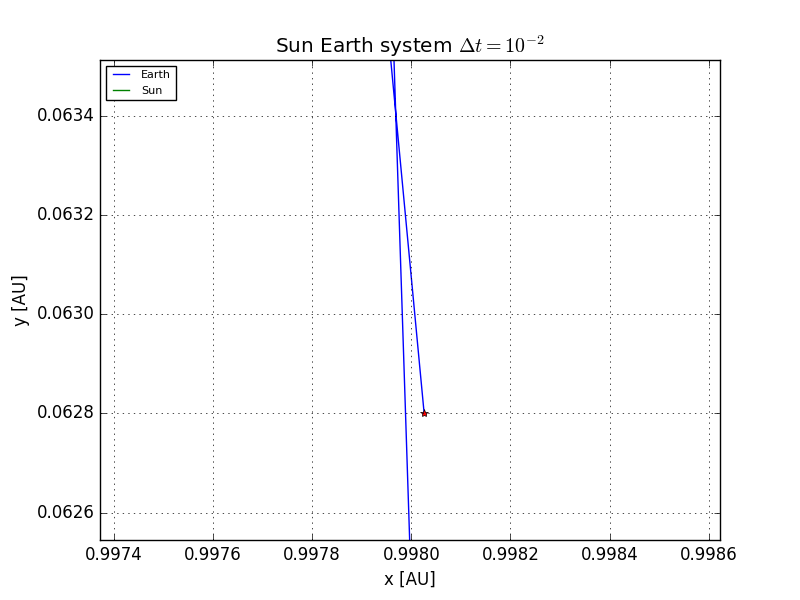
\includegraphics[height=2.0in]{orbitESe2y2png.png}
        \caption{Close-up of timestep of $10^{-2}$}
    \end{subfigure}%
    ~ 
    \begin{subfigure}[H!]{0.5\textwidth}
        \centering
        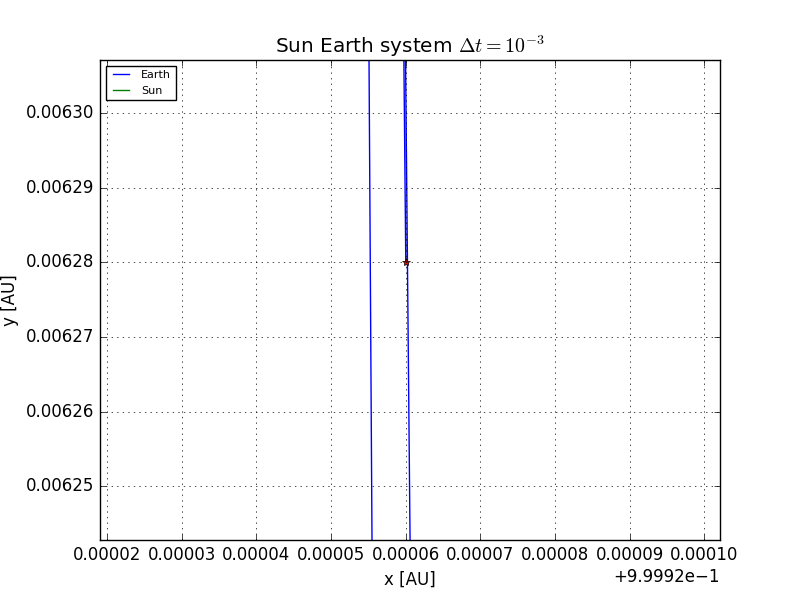
\includegraphics[height=2.0in]{orbitESe3y2png.png}
        \caption{Close-up of timestep of $10^{-3}$}
    \end{subfigure}
    \caption{Plot of the earth-sun system for different time steps of the simulation. These simulations are run over 2 years.}\label{fig:timestep}
\end{figure}

\subsubsection{Investigating the required escape velocity}
The plot for the earth-sun system with the initial velocity of the earth slightly varied is shown below.
\begin{figure}[!ht]
    \centering
    \begin{subfigure}[H!]{0.5\textwidth}
        \centering
        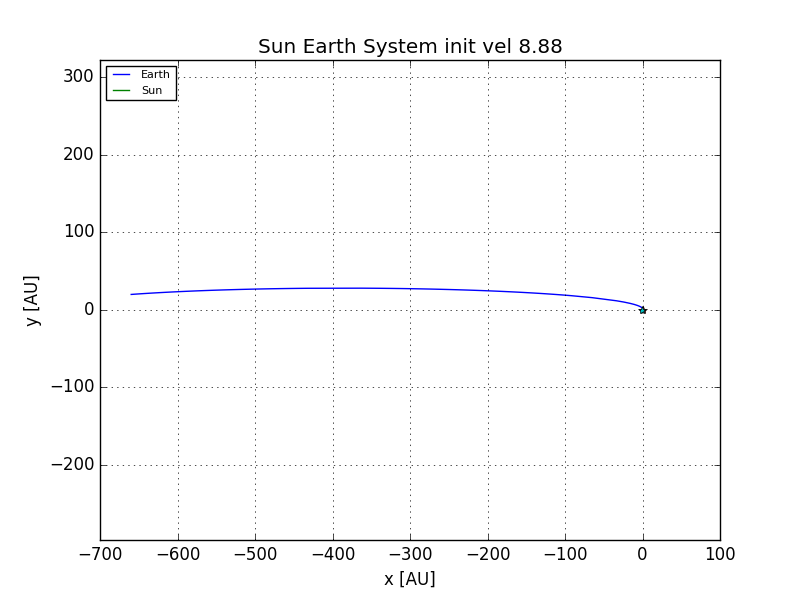
\includegraphics[height=2.0in]{escape888.png}
        \caption{Initial velocity of 8.88 AU/yr}
    \end{subfigure}%
    ~ 
    \begin{subfigure}[H!]{0.5\textwidth}
        \centering
        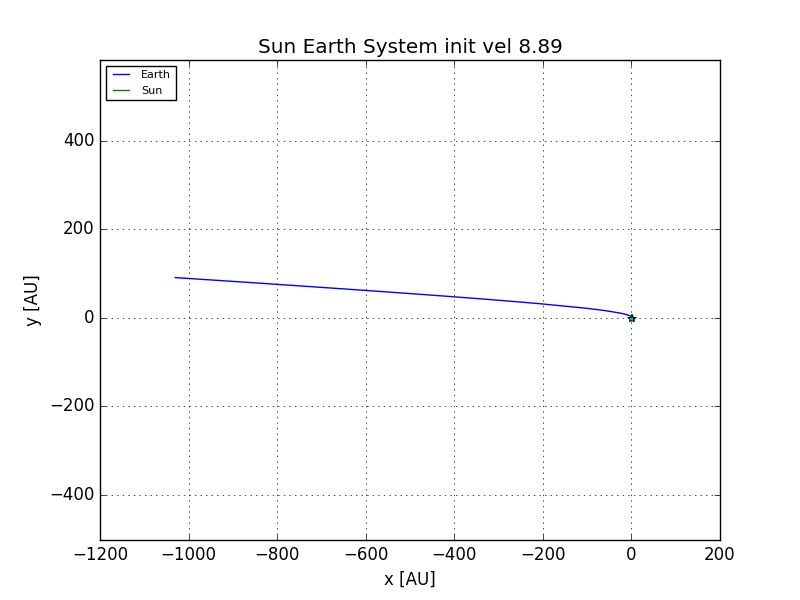
\includegraphics[height=2.0in]{escape889.png}
        \caption{Initial velocity of 8.89 AU/yr}
    \end{subfigure}
    \caption{Plot of the earth-sun system for different initial velocities. The simulation runs for 2000 years, with $10^5$ timesteps per year.}\label{fig:escape_vel}
\end{figure}
\newpage
\subsection{Results from the second model-Earth, Jupiter and Sun}
\subsubsection{Position}
The orbit of the three-body system consisting of the earth, Jupiter and the sun is shown below. We have also included a zoomed in version of the same plots.
\begin{figure}[!ht]
    \centering
    \begin{subfigure}[H!]{0.5\textwidth}
        \centering
        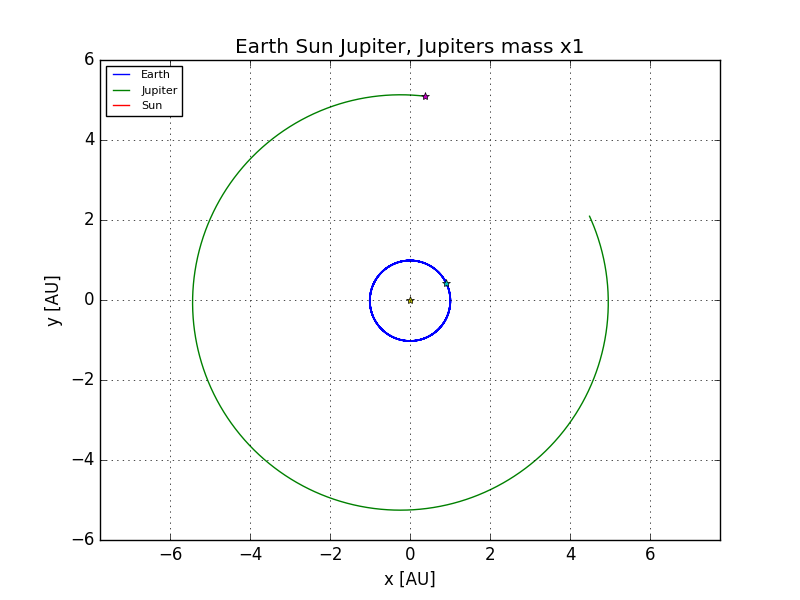
\includegraphics[height=2.0in]{orbitESJ1.png}
        \caption{Jupiter with original mass}
    \end{subfigure}%
    ~ 
    \begin{subfigure}[H!]{0.5\textwidth}
        \centering
        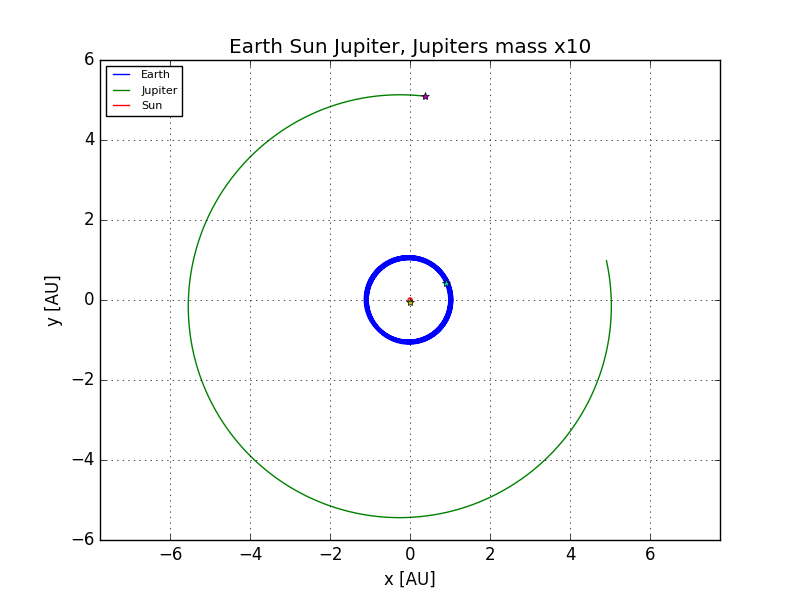
\includegraphics[height=2.0in]{orbitESJ10.png}
        \caption{Jupiter with mass ten times its original mass}
    \end{subfigure}
    \caption{Sun, Earth and Jupiter system for different masses of Jupiter. Notice the larger deviations in Earth's orbit (thicker line).} \label{fig:jupiter1-10}
\end{figure}
We wanted to do a similar thing for the mass of Jupiter being 1000 times larger than it is in reality, but here we ran into a problem. If we let the center of mass be at the origin, with zero velocity, the earth crashes into Jupiter. When we let the sun be at the origin, however, we get a chaotic system, but without crashes. We have therefore included both of these possibilities.

\begin{figure}[!ht]
    \centering
    \begin{subfigure}[H!]{0.5\textwidth}
        \centering
        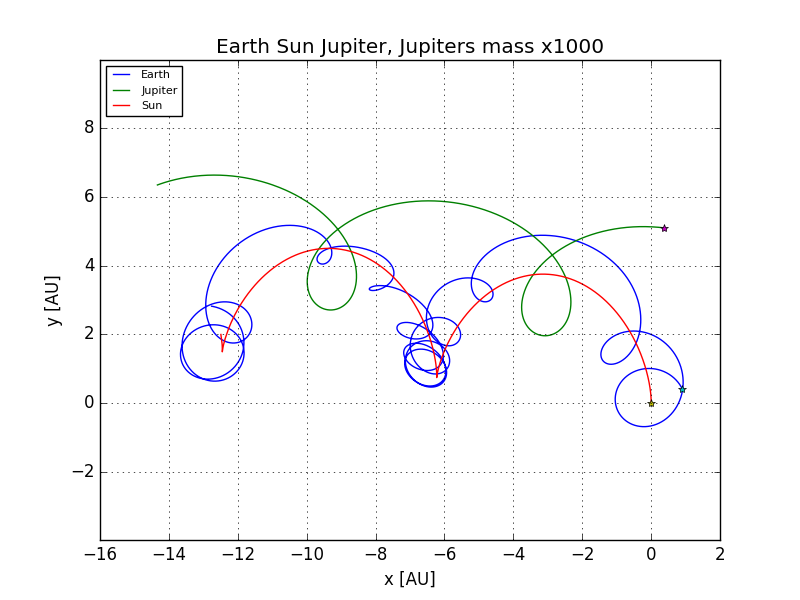
\includegraphics[height=2.0in]{orbitESJ1000.png}
        \caption{Jupiter at 1000 times its original mass, sun at the origin with zero initial velocity}
    \end{subfigure}%
    ~ 
    \begin{subfigure}[H!]{0.5\textwidth}
        \centering
        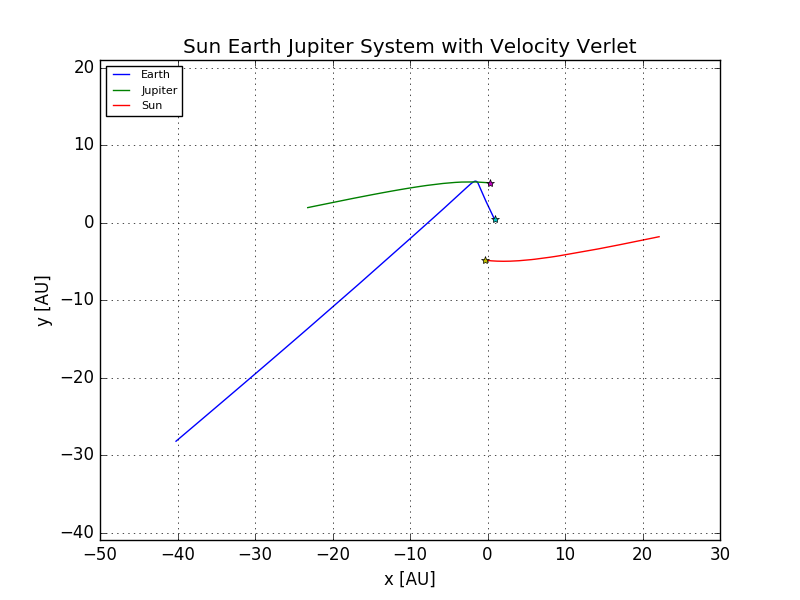
\includegraphics[height=2.0in]{orbitSEJMCAtOri.png}
        \caption{Jupiter at 1000 times its original mass, center of mass at origin with zero velocity.}
    \end{subfigure}
    \caption{Sun, Earth and Jupiter system with Jupiter's mass increase by a factor 1000. The stars indicate the initial positions of the objects. We simulate for 10 years, with $10^5$ timesteps per year. Notice how earth crashes into Jupiter in subplot b.}\label{fig:Jupiter1000}
\end{figure}
\newpage
\subsubsection{Conservation of energy and angular momentum per unit mass}
A plot of the relative error in the total energy and the total angular momentum per unit mass for Jupiter's mass equal to 10 and 1000 is shown below. We did not include the plot for the situation where the center of mass is not at the origin with initial velocity, as the center of mass will be moving in this case, and we have taken the angular momentum relative to a fixed point. Thus angular momentum is not necessarily conserved in that case.
\begin{figure}[!ht]
    \centering
    \begin{subfigure}[H!]{0.5\textwidth}
        \centering
        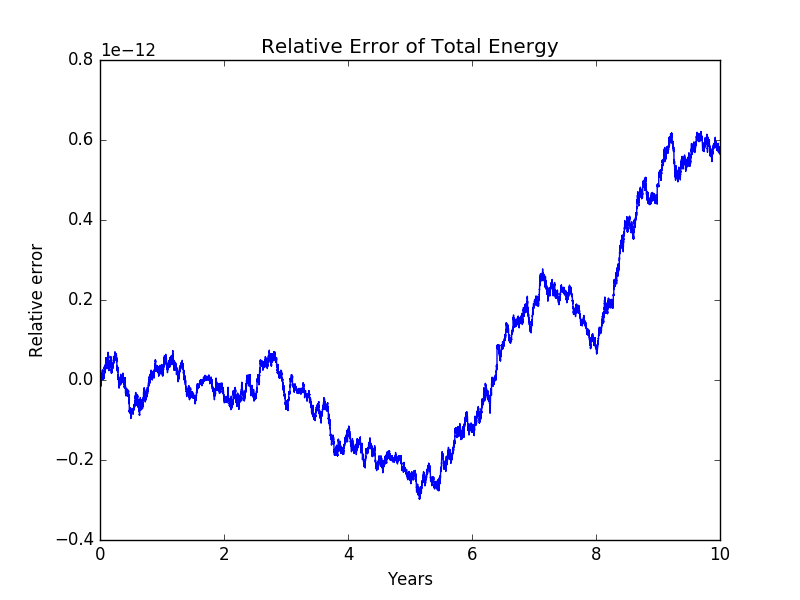
\includegraphics[height=2.0in]{relErrEnSEJx10.png}
        \caption{Relative error in the total energy.}
    \end{subfigure}%
    ~ 
    \begin{subfigure}[H!]{0.5\textwidth}
        \centering
        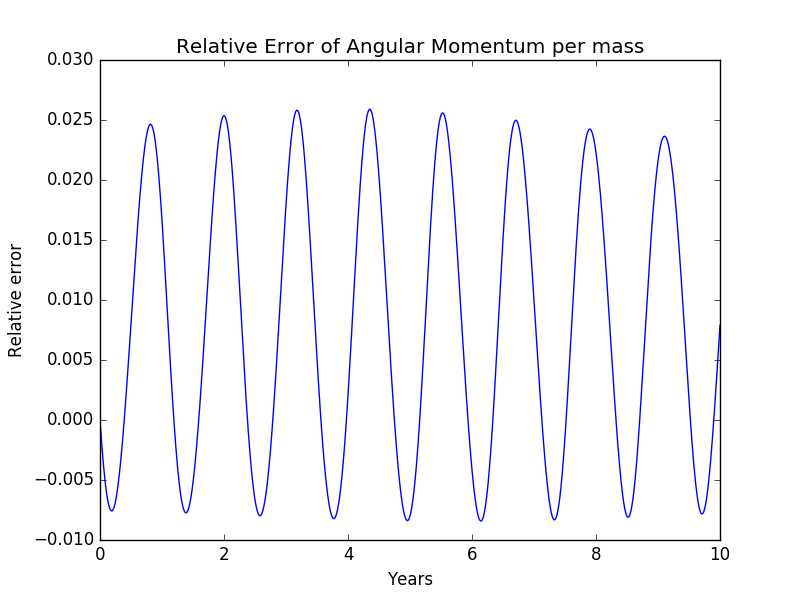
\includegraphics[height=2.0in]{relErrMomSEJx10.png}
        \caption{Relative error in the total angular momentum per unit mass.}
    \end{subfigure}
    \caption{Variations in the error of the total energy and the total angular momentum per unit mass for the Earth, Sun and Jupiter system. The mass of Jupiter is 10 times higher than its actual mass, and the simulation are run for 10 years, with $10^5$ time steps per year.}\label{fig:Energy_jupiter_10}
\end{figure}
\begin{figure}[!ht]
    \centering
    \begin{subfigure}[H!]{0.5\textwidth}
        \centering
        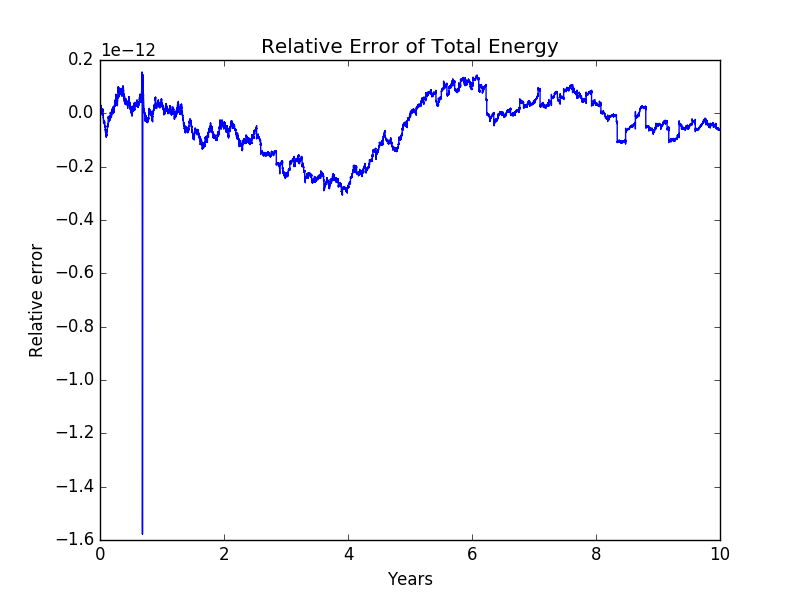
\includegraphics[height=2.0in]{relErrEnSEJ.png}
        \caption{Relative error in the total energy.}
    \end{subfigure}%
    ~ 
    \begin{subfigure}[H!]{0.5\textwidth}
        \centering
        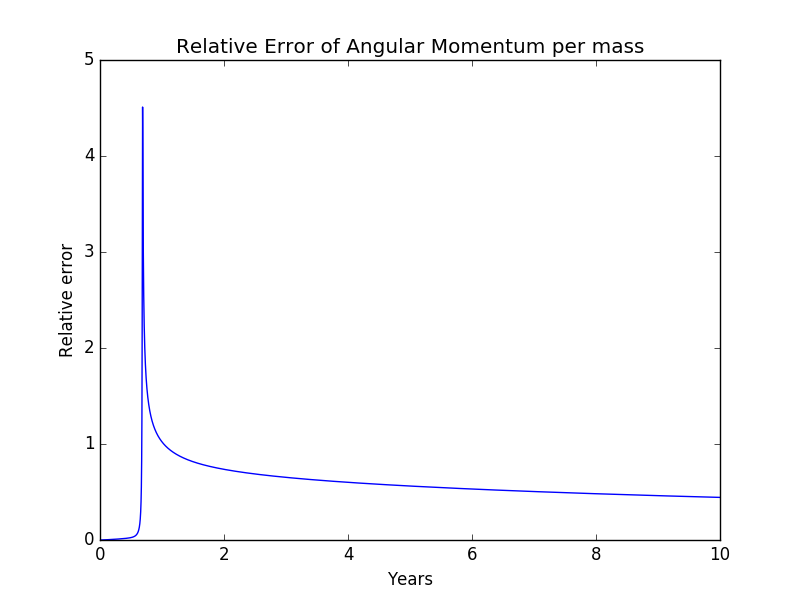
\includegraphics[height=2.0in]{relErrMomSEJ.png}
        \caption{Relative error in the total angular momentum per unit mass.}
    \end{subfigure}
    \caption{Variations in the error of the total energy and the total angular momentum per unit mass for the Earth, Sun and Jupiter system. The mass of Jupiter is 1000 times higher than its actual mass, and the simulation are run for 10 years, with $10^5$ time steps per year. The center of mass is at the origin with zero velocity.}\label{fig:Energy_jupiter_1000}
\end{figure}
\newpage

\subsection{Results from the third model - Entire Solar System}
\subsubsection{Position}
A plot of the entire solar system is shown in the figures below. We have also included a zoomed in version, to illustrate the orbit of the closest planets.
\begin{figure}[!ht]
    \centering
    \begin{subfigure}[H!]{0.5\textwidth}
        \centering
        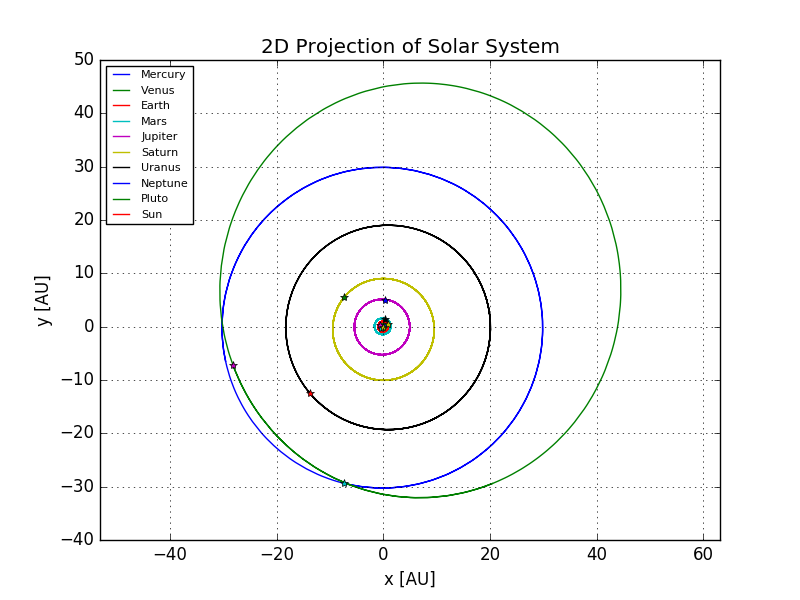
\includegraphics[height=2.0in]{orbitfull.png}
        \caption{Position of all planets}
    \end{subfigure}%
    ~ 
    \begin{subfigure}[H!]{0.5\textwidth}
        \centering
        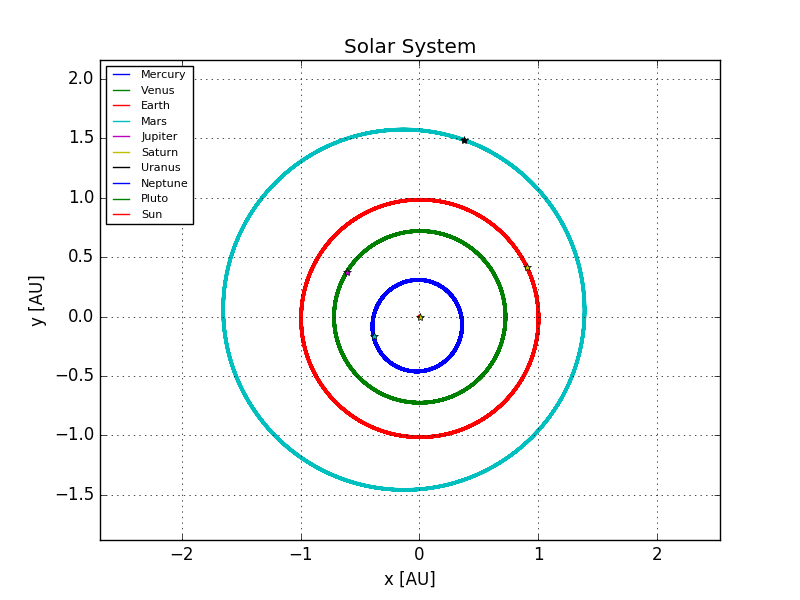
\includegraphics[height=2.0in]{orbitFull.png}
        \caption{Zoomed in plot, showing only the innermost planets}
    \end{subfigure}
    \caption{Plot of the entire solar system, as well as a zoom on the innermost planets. This was produced with $10^5$ steps per year, running the simulation for a total of 300 years.} \label{fig:solar_system}
\end{figure}
\subsubsection{Conservation of energy and angular momentum per unit mass}
A plot of the relative error in the total energy and the total angular momentum per unit mass for the entire solar system is shown below:
\begin{figure}[!ht]
    \centering
    \begin{subfigure}[H!]{0.5\textwidth}
        \centering
        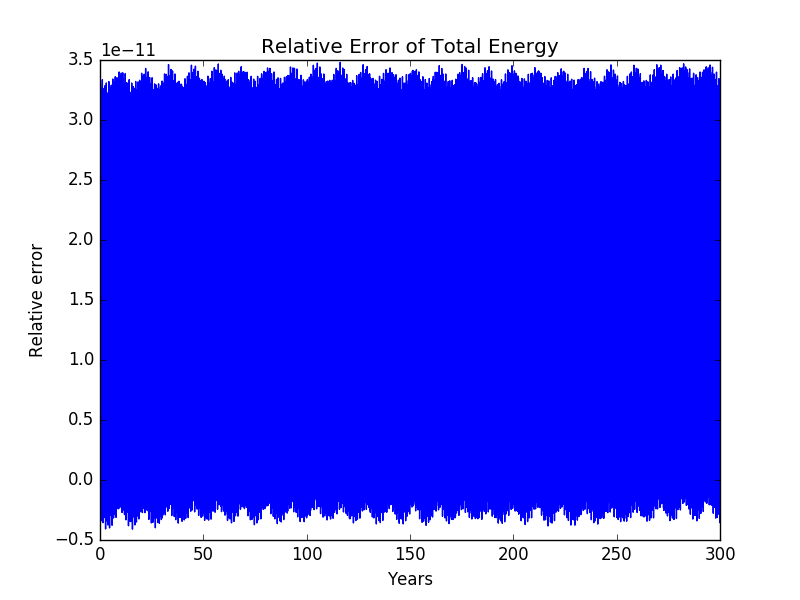
\includegraphics[height=2.0in]{relErrEnFull.png}
        \caption{Relative error in the total energy}
    \end{subfigure}%
    ~ 
    \begin{subfigure}[H!]{0.5\textwidth}
        \centering
        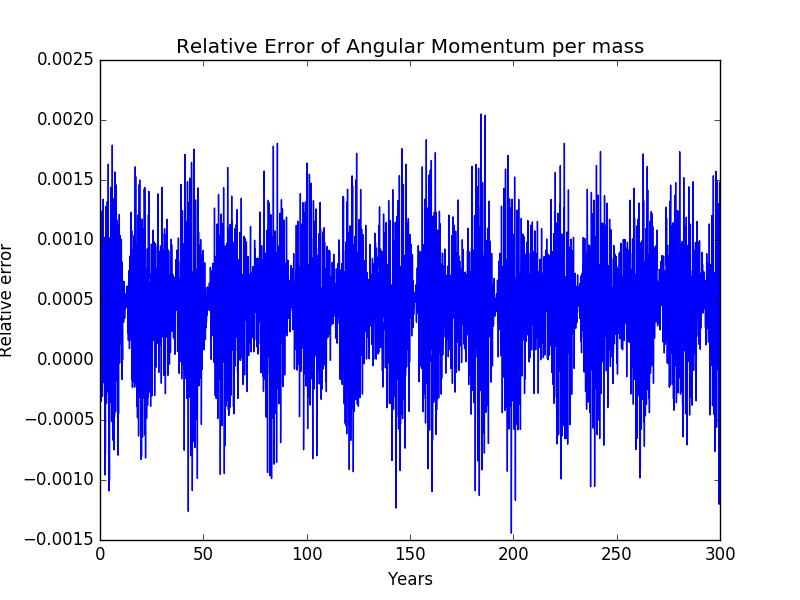
\includegraphics[height=2.0in]{relErrMomFull.png}
        \caption{Relative error in the total angular momentum per unit masss}
    \end{subfigure}
    \caption{Relative error of conserved quantities for the entire solar system.} \label{fig:error_full_solar_system}
\end{figure}
\newpage

\subsection{Results from the fourth model - Mercury-Sun System}
\subsubsection{Position}
For this system, we plot the variation in the perihelion angle with and without Newtonian gravity below:
\begin{figure}[!ht]
    \centering
    \begin{subfigure}[H!]{0.5\textwidth}
        \centering
        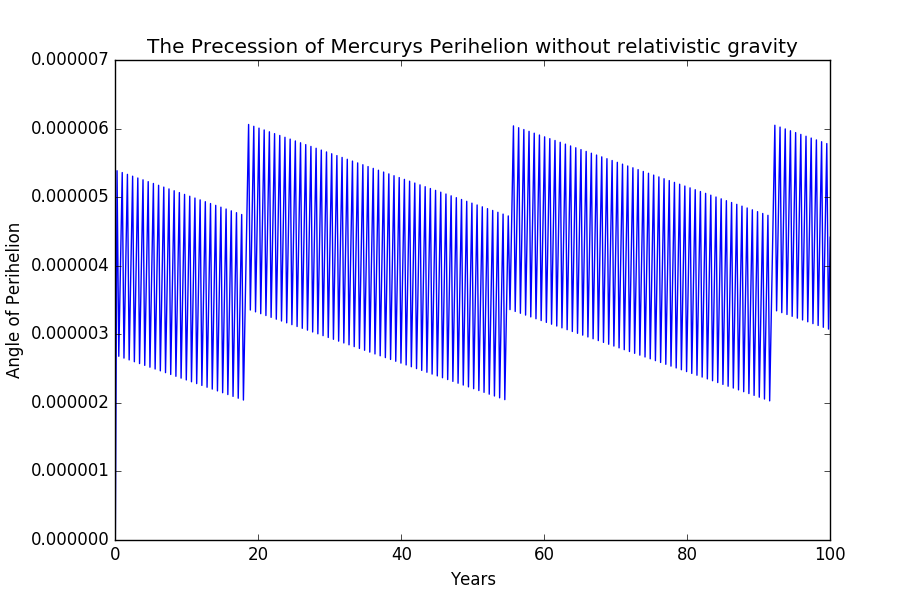
\includegraphics[height=2.0in]{angleNoRel2.png}
        \caption{Newtonian gravity}
    \end{subfigure}%
    ~ 
    \begin{subfigure}[H!]{0.5\textwidth}
        \centering
        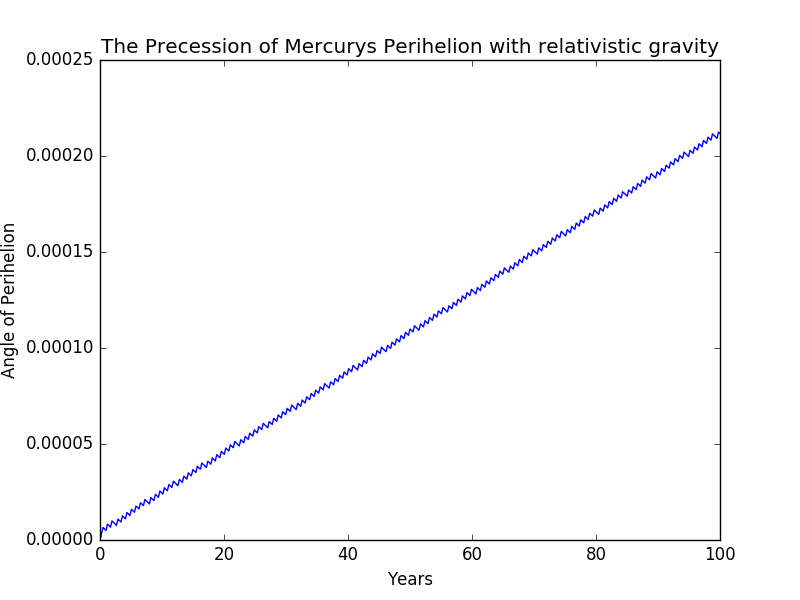
\includegraphics[height=2.0in]{angle.png}
        \caption{Relativistic gravity}
    \end{subfigure}
    \caption{Plot of the variation of the perihelion angle over a century, using both the Newtonian and the relativistic expressions for gravity. Here we employed a higher precision of $10^7$ steps per year, because the variations in angle are so small.} \label{fig:precession}
\end{figure}
\newpage
\section{Discussion}
In this section we discuss the results from the previous section for the various models.
\subsection{Interpreting the results from the Earth-Sun model}
\subsubsection{Choice of algorithm}
\paragraph{Position graphs:}
The earth-sun model, whilst simple, provides us with important insight into the details of our solvers. Note how both the Euler forward algorithm and the Velocity-Verlet algorithm produce acceptable result without too much computational power (only about 0.8 seconds for the Euler forward algorithm and just over 1 second for the Velocity-Verlet algorithm). It is clear, however, that the Velocity-Verlet is significantly better. As can be seen in \cref{fig:earth-sun-figure1}, even when the zoom is increase by a factor ten when compared with the Forward Euler, it is not possible to distinguish between the transits.
\paragraph{Conservation of energy} 
Another important argument comes from observing the energy. Notice how the error in relative energy and angular momentum per unit mass varies systematically for the Forward Euler algorithm. The relative error of the energy is always negative and decreasing. Notice that, from section \ref{conservation_of_energy}, the energy must always remain negative if potential energy is to be greater than kinetic energy, and the earth is to remain gravitationally bound. Thus, when calculating the relative error, in equation \ref{eq:relative_error}, we are subtracting two negative numbers and then dividing by another negative number. If this is negative, this means that initial energy is less than the energy at a time $t$. Thus the energy is increasing with time. This also explains the trend of the relative error in angular momentum per unit mass. Notice how this error is increasing as time, which means that angular momentum per unit mass is increasing with time. Thus, it seems that velocity, and therefore kinetic energy and angular momentum per unit mass,  is increasing with time. It is not entirely obvious why the forward Euler algorithm would do this. The forward Euler is biased, as it computes the position based only on the forward velocity estimate, ignoring the velocity of the last time step. This does not entirely explain the observed trend however.\\
\linebreak
Notice how total energy and the total angular momentum per unit mass follow the same pattern for the Velocity-Verlet method (a negative relative error in the energy corresponds to a positive error of the angular momentum), but there is no clear bias - there are oscillations and seemingly random movements. Furthermore, the magnitudes of the errors are \textit{significantly} lower than the errors for the Forwad Euler algorithm.\\
\linebreak
\linebreak
All these factors together justify our choice to use the Velocity-Verlet method for the rest of the investigation.
\subsubsection{Choice of time step}
As can be seen from \cref{fig:timestep}, for $\Delta t=10^{-2}$ and $\Delta t= 10^{-3}$, the results are rather poor - the deviations are apparent at a scale of $10^{-3}$ AU. For $\Delta t= 10^{-4}$ this was significantly better for the simple earth-sun system,but this broke down for the more complex system. For $\Delta t = 10^{-5}$, matplotlib would not let us zoom in close enough to see any deviations. Whilst these deviations are undoubtedly there (as can be seen from the fact that we used significantly larger time steps when searching for the perihelion angle), we decided to keep $\Delta t = 10^{-5}$, i.e. $10^5$ timesteps per year, for most of the simulations, as it appeared to strike an acceptable balance between CPU time and precision.
\subsubsection{Escape velocity}
As can be seen in \cref{fig:escape_vel}, our simulation seems to reproduce the expected escape velocity. Careful inspection of the plot reveals a curving for the lower velocity. This clearly indicates an elliptical orbit. For the higher velocity, this curving is not present, which indicates that this is a parabolic (or mayhap hyperbolic) escape. This is a reassuring check for the consistency of our system, and it confirms that our choice of $\Delta t$ is justified
\subsection{Interpreting the results from the Earth, Sun and Jupiter model}
\subsubsection{The orbits of the planets}
It is reassuring to see, as shown in \cref{fig:jupiter1-10} a), that our system still appears to be stable with the most massive planet in the solar system added. On the scale shown, there are no visible deviations from the earlier plot, and even when zooming these deviations are hard to see. This shows that the sun is the utterly dominating object in the solar system.\\
\linebreak
For the case when Jupiter is 10 times heavier, we can seem from \cref{fig:jupiter1-10} b) that Earth's orbit becomes thicker - the earth wobbles. A zoomed in version of the same image is shown below:
\begin{figure}[!ht]
    \centering
    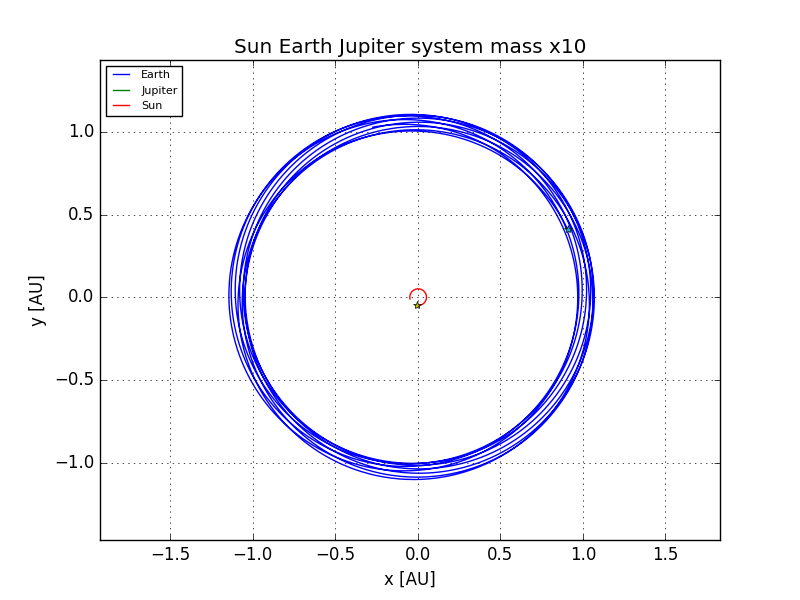
\includegraphics[height=2.5in]{orbitESJ10Close.png}
    \caption{A zoomed in version of \cref{fig:jupiter1-10} b).}
\end{figure}
\linebreak
This shows that earth's orbit is moving slightly back and forth, due to the tidal forces from Jupiter. Nonetheless, it is clear that the sun is still the dominating body in this case.\\
\linebreak
For the case where Jupiter is 1000 times heavier than in reality, things break down slightly. Here, the mass of Jupiter is comparable to the mass of the sun, and consequently this turns into a chaotic three-body problem. It is interesting to observe that the system keeps together in an oscillating state when the sun starts at the origin, whilst it flies apart if the center of mass starts at the origin. This illustrates the complex and frequently unstable behavior of three-body systems. 
\subsubsection{Energy and angular momentum per unit mass in the Earth, Sun and Jupiter system}
The energy in the system where Jupiter's mass is increased by a factor 10 is shown in \cref{fig:Energy_jupiter_10}. This shows a similar pattern to the energy in the Earth-Sun system. The energy fluctuates slightly, and the errors seems to increase over time, but the fluctuations are minuscule. The relative error of the angular momentum per unit mass, on the other hand, displays a different behavior - it oscillates periodically, with a non-negligible amplitude. This is a behavior which we observed in any system containing the two heaviest planets. It is not entirely obvious why this fluctuations occur, though the most likely explanation is that the center of mass moves periodically, due to the gravitational effects of the heaviest planets, perhaps due to an accidental incorrect initialization of the center of mass. Oddly, however, this effect seemed to persist even when the time step was lowered significantly. This may be a potential source of future investigation. One particularly interesting aspect of this is the fact that the oscillations do not have a mean of zero, but are biased towards positive values. This could indicate that the center of mass has a tendency to move so that the angular momentum relative to the origin increases. It is not obvious why this occurs.\\
\linebreak
The angular total energy and angular momentum per unit mass for the case where Jupiter is 1000 times heavier than in reality are shown in \cref{fig:Energy_jupiter_1000}. This is for the case where the center of mass is at the origin and does not move (so that the angular momentum, taken relative to the origin, should be constant). Here our model clearly break down.This is presumably due to the fact that the earth crashes into Jupiter. As we have excluded collision detection in our algorithm, numerical errors may have increase considerably, as the velocity of the earth changes rapidly in a single time step. Thus, these results are not representative of the underlying physics, and we do not discuss them further.
\subsection{Interpreting the results from the full solar system}
\subsubsection{The orbit in the solar system}
The orbits are shown in figure \cref{fig:solar_system}. Note that these are two-dimensional projections of the orbit. An animated version of both the 2D and 3D orbits can be found on our \href{https://github.com/dulte/Comp-Phys/tree/master/Project3Final}{GIT page}\footnote{https://github.com/dulte/Comp-Phys/tree/master/Project3Final}. As can be seen there, the orbits are almost entirely coplanar, except for the orbit of Pluto. Notice how the oribts are stable for 300 years, though the innermost orbits show some variations - both due to numerical errors and due to the effects of the more massive planets. In general, however, the Verlet method seems stable over 300 years, with the given time step. Note that these simulations only took about 20 seconds to run. This indicates that the Verlet algorithm is quite stable at our chosen time step.
\subsubsection{Conservation of energy angular momentum per unit mass}
As shown in \cref{fig:error_full_solar_system}, the oscillations of the relative error in the total energy are still minuscule but, interestingly, not with a mean of zero. The total angular momentum per unit mass shows a similar oscillating behavior as previously, but with a larger ensemble of frequencies. The reason is presumably the same as in the previous model - a moving center of mass. Whilst angular momentum should be conserved, it must be calculated relative to a point numerically. We calculated angular momentum with respect to the origin, however, if that is not where the center of mass is, and if the center of mass has a nonzero velocity, we may get deviations. These may explain the above behavior though they, as earlier, do not explain why there would be a non-zero mean.
\subsection{Discussing the perihelion precession of mercury}
We show the perihelion angle of Mercury with Newtonian gravity in \cref{fig:precession} a). This angle is not exactly zero, contrary to what one may expect. Because of the discretization of the position of Mercury, its closed distance to the sun will rarely be at the exact perihelion. Instead, our algorithm will tend to over- or undershoot the perihelion. We therefore expect the angle to oscillate around zero. By considering the amplitude of the oscillation,  we see that the numerical error of the angle is of the order $10^{-6}$. If we factor out this error we expect to get a constant angle of 0. But doing this with the data in \cref{fig:precession} a) gives a constant angle of $\sim 4 \cdot 10^{-6}$. We are not sure of the reason for this discrepancy, but below we shall argue that this error is so small that it can be ignored. Even with the discrepancy of $\sim 4 \cdot 10^{-6}$, the angle is more or less constant over a century, meaning that Newtonian gravity fails to give the 43 arcsec or $0.0002085$ rad precession of the angle that we expect from observations. \linebreak

\cref{fig:precession} b) shows that relativistic gravity no longer gives us a constant angle of the perihelion, but instead a constant precession. To try to eliminate the discrepancy in the angle of $\sim 4 \cdot 10^{-6}$, we don't look at the value of the angle after a century, but take the difference of the endpoints, giving us a precession of the angle of $0.00020841$ or $42.9876"$, which gives $0.3\%$ relative error from the analytic result. \\

The difference between the Newtonian and relativistic angle is of the magnitude $-4$, meaning that it is 100 times larger than the error we got due to the discretization of position. This means that with this error we can be sure of the restults within $\pm 1\%$. With a relative error of $0.3 \%$, our result was within this range, and we can conclude that our result gives evidence that general relativity gives a better description of gravitation than Newtonian gravity. Thus our algorithm was able to reproduce this result.
\section{Conclusion and outlook}
\subsection{Conclusion}
We have shown that the Verlet solver works well for our chosen parameters,as it reproduces a stable solar system. We have also shown that the Verlet solver is far superior to the forward Euler algorithm. This illustrates that, when solving complex coupled differential equations numerically, the choice of methods and parameters is crucial. We have also investigated how well our model reproduces the expected escape velocity for earth, and the perihelion precessions of mercury predicted by general relativity. We found that our model reproduces both of these results to an acceptable precision.\\
\linebreak
We did have some rather odd behavior for the angular momentum per unit mass and the conservation of energy for some of our models. The fluctuations were small, however, and did not impact our results significantly. Nonetheless, this seems to be an indication of an error somewhere, as the periodic change in the relative error goes against physical intuition and theoretical predictions. 
\subsection{Outlook}
There is much further work which could be put into this project. Most interestingly, perhaps, would be to explain the periodic behavior of the angular momentum. One way to approach this may be to calculate the position of the center of mass at every time step, and subsequently taking the angular momentum relative to this, to ensure that angular momentum is always taken relative to the center of mass as it was initially. If the center of mass moves for any reason (such as numerical errors), and the calculations do not take this into account, there may be an unexpected torque on the system.\\
\linebreak
Another interesting future topic may be to investigate the behavior of the forward Euler algorithm further, in particular why it produces linear graphs for the relative error. This is not entirely obvious, and may be interesting.\\
\linebreak
Finally, it may be very rewarding to have a closer look at the three-body problem posed by Jupiter being 1000 times heavier. As can be seen from \cref{fig:Jupiter1000}, the behavior of the system is stunning, and may well be worth investigating further.
\addcontentsline{toc}{section}{References}
\bibliography{Project3}
\bibliographystyle{apalike}
\newpage
\begin{appendices}
\section{Initial velocity for circular orbits and the value of G}\label{ap:Find_Circular_orbit}
If we assume a two-body system, consisting of the earth and the sun, transform to a system where the sun's velocity is zero, and assume circular orbit, we can equate the force of gravity to the centripetal force. For the earth this gives:
$$\frac{GM_{\odot}m_e}{r^2}=m_e\frac{v_{circ}^2}{r}$$
Where $m_e$ is the mass of earth. Rearranging gives:
\begin{equation}\label{eq:Vel_for_cicrular_orbit}
v_{circ}=\sqrt{\frac{GM_{\odot}}{r}}
\end{equation}
Inserting $r=1 \mathrm{AU}$ gives for the earth $v_{circ}=29\ 780$. This is the velocity we must give the earth (in a frame where the initial velocity of the sun is zero)\footnote{We will use this value as initial velocity of the earth in the earth-sun system, even though we give the sun an additional velocity to ensure that the center of mass does not move. It is clear that these differences will be minuscule, and doing this otherwise would result in a complicated dynamic problem.}, to ensure that it orbits in a circular orbit of radius $1 \mathrm{AU}$. 
\linebreak
From this equation, we can also find a value for $G$ in the units astronomical units per year. We simply say that the earth takes one year to complete one revolution, which gives $v_{circ}=2\pi r/T=2\pi \ \mathrm{AU/yr}$. Solving equation \ref{eq:Vel_for_cicrular_orbit} for $G$ gives:
$$G=\frac{v_{circ}^2 r}{M_{\odot}}$$
Seeing as  $r=1 \ \mathrm{AU}$, this gives:
$$G=4\pi^2\ \ \mathrm{AU^3}\mathrm{yr^{-2}M_{\odot}^{-1}}$$
Which also shows that $v_{circ}=2\pi \ \mathrm{AU/yr}$.
\section{Deriving the Velocity-Verlet algorithm}\label{ap:Deriving_VelVer}
Here will derive the Velocity-Verlet method. We will derive this for a single dimension ($x$), however the three-dimensional generalization is straightforward, as it simply amounts to repeating the exact same equation with $x$ exchanged with $y$ and $z$ respectively.\\
\linebreak
The Velocity-Verlet method is based on Taylor-expanding the acceleration, $a$, around $x=x_0$. This gives:
$$a(x_0+h)=a(x_0)+ha'(x_0)+O(h^2)$$
Or, discretizing as described in section \ref{discretize_equations}, gives approximately:
$$a_{i+1}\approx a_i+ha'_i$$
Or, rearranging slightly:
\begin{equation} \label{eq:discretized_acceleration}
ha_i'\approx a_{i+1}-a_i
\end{equation}
Now we expand the velocity in the same way, but include another term in the Taylor expansion. This gives:
$$v_{i+1}= v_i+ha_i+\frac{h^2}{2}a'_i+O(h^3)$$
Inserting from equation \ref{eq:discretized_acceleration} gives:
$$v_{i+1}=v_i+a_ih+\frac{h}{2}\left(a_{i+1}+a_i\right)+O(h^3)$$
Finally, we Taylor expand the position in the same way to get:
$$x_{i+1}=x_i+hv_i+\frac{h^2}{2}a_i+O(h^3)$$
These are the equations of the Velocity-Verlet algorithm described in equation \ref{eq:Vel_Ver_eq}. Notice how the error is proportional to $h^3$, as opposed to the Forward-Euler algorithm, where the error is proportional to $h^2$.

\end{appendices}
\newpage
\end{document}

